\documentclass[a4paper,12pt]{report}
\usepackage{sethesis}
\usepackage{amsmath}
\usepackage{amsfonts}
\usepackage{amssymb}
\usepackage[ngerman]{babel}
\usepackage{graphicx}
\usepackage{caption}
\usepackage{subcaption} 
\usepackage{hyperref}
\usepackage{float}
\usepackage{hyphenat}
\usepackage{subfiles}
\usepackage{multirow}
\usepackage{tabularray}
\usepackage{listings}
\usepackage{xcolor}
\usepackage{array}
\usepackage{colortbl}

\definecolor{codegreen}{rgb}{0,0.6,0}
\definecolor{codegray}{rgb}{0.5,0.5,0.5}
\definecolor{codepurple}{rgb}{0.58,0,0.82}
\definecolor{backcolour}{rgb}{1,1,1}

\lstdefinestyle{mystyle}{
  backgroundcolor=\color{backcolour},   
  commentstyle=\color{codegreen},
  keywordstyle=\color{magenta},
  numberstyle=\tiny\color{codegray},
  stringstyle=\color{codepurple},
  basicstyle=\ttfamily\footnotesize,
  breakatwhitespace=false,         
  breaklines=true,                 
  captionpos=b,                    
  keepspaces=true,                 
  numbers=left,                    
  numbersep=5pt,                  
  showspaces=false,                
  showstringspaces=false,
  showtabs=false,                  
  tabsize=2
}

\title{CPU - Steuerwerk}
\unilogo{
\includegraphics[scale=0.75]{FHDW-Logo.eps}}

\myauthor{
  Kurs HFI423
}
\version{v1.0.0}

\studiengang{Informatik}
\ort{Hannover}
\datum{\today}



\begin{document}

\maketitle

\clearpage

\tableofcontents



\chapter{Einleitung}
\label{chap:einleitung}

Das Steuerwerk nimmt Befehle aus dem Hautspeicher entgegen, decodiert diese und erzeugt daraus eine geeignete zeitliche Sequenz von
Steuersignalen für das Rechenwerk. Neben der ALU ist dies ein Hauptbestandteil eines Prozessors.

\chapter{Aufbau und Funktion der CPU}
\label{chap:Aufbau und Funktion der CPU}





\chapter{Steuerwerk}
\label{chap:Steuerwerk}

\section{Allgemeine Funktion}

Das Steuerwerk ist das zentrale Element der CPU, das für die Koordination aller Komponenten verantwortlich ist.
Es erzeugt die Steuersignale, um Datenflüsse und Operationen innerhalb der Architektur zu steuern.
Außerdem kontrolliert es den Programmzähler (PC) und verwaltet die Adressierung von Befehlen und Daten im RAM.
\\\\
Das Steuerwerk erhält Statussignale (z. B. Carry, Overflow, Zero), die von der ALU generiert werden, und
passt die Steuerung an, um Instruktionen korrekt auszuführen.
\\\\
Im Folgenden werden die Ein- und Ausgänge des Steuerwerks detailliert beschrieben.

\section{Eingänge}
\begin{table}[H]
    \centering
    \begin{tabular}{|l|p{10cm}|}
        \hline
        \textbf{Signal}   & \textbf{Beschreibung}                                                           \\ \hline
        \textbf{Reset}    & Setzt das Steuerwerk in den Anfangszustand zurück.                              \\ \hline
        \textbf{BLA}      & Busy-Look-Ahead-Signal zur Vorhersage von Busy-Zuständen in der ALU.            \\ \hline
        \textbf{Busy}     & Statussignal der ALU, das die ALU momentan mit einer Operation beschäftigt ist. \\ \hline
        \textbf{Carry}    & Flag, das von der ALU bei einem Übertrag (Carry) gesetzt wird.                  \\ \hline
        \textbf{Overflow} & Flag, das bei einem Überlauf (Overflow) während ALU-Operationen gesetzt wird.   \\ \hline
        \textbf{Zero}     & Flag, das gesetzt wird, wenn das ALU-Ergebnis null ist.                         \\ \hline
        \textbf{C3..0}    & Die von der ALU auszuführende Operation.                                        \\ \hline
    \end{tabular}
    \caption{Eingänge des Steuerwerks}
\end{table}

\noindent Die Flags werden in \autoref{TODO} ausführlich erklärt.
\\\\
Die genannten Eingänge sind nötig für die Entscheidung, welche Operation als nächstes durchgeführt wird. \\
Das Steuerwerk nutzt diese Signale, um Befehle effektiv zu koordinieren und auszuführen und generiert die im folgenden Abschnitt aufgeführten Ausgaben.

\section{Ausgänge}
\begin{table}[H]
    \centering
    \begin{tabular}{|l|p{10cm}|}
        \hline
        \textbf{Signal}      & \textbf{Beschreibung}                                                                                           \\ \hline
        \textbf{WriteA}      & Schreibt Operanden aus dem RAM in Register A.                                                                   \\ \hline
        \textbf{WriteRAM}    & Schreibt das Ergebnis von Register A in den RAM.                                                                \\ \hline
        \textbf{WriteADR1}   & Speichert die 4 MSB-Adressbits (ADR7..4) aus dem RAM im Adressregister (RegADR).                                \\ \hline
        \textbf{WriteADR2}   & Speichert die 4 LSB-Adressbits (ADR3..0) aus dem RAM im Adressregister (RegADR).                                \\ \hline
        \textbf{WriteOP}     & Schreibt die aktuelle Operation in das OpReg während des Fetch-Zyklus.                                          \\ \hline
        \textbf{!PC\_LD}     & Lädt den Programmzähler (PC).                                                                                   \\ \hline
        \textbf{!PC\_EN}     & Aktiviert den Programmzähler, damit er hoch- oder runterzählen kann.                                            \\ \hline
        \textbf{PC\_UP}      & Gibt an, ob der PC hochzählt (\texttt{PC\_UP=1}) oder runterzählt (\texttt{PC\_UP=0}).                          \\ \hline
        \textbf{RegADRtoRAM} & Bestimmt, ob die Adresse im RAM von RegADR oder dem Programmzähler kommt. Bei \texttt{RegADRtoRAM = 1}
        Wird die Adresse vom RegADR übertragen.                                                                                                \\ \hline
        \textbf{ALUStart}    & Startet die ALU zur Ausführung einer Operation.                                                                 \\ \hline
        \textbf{SWR}         & Tauscht den Inhalt von Register A und Register B, die beim Starten der ALU die Operanden in die ALU übertragen. \\ \hline
    \end{tabular}
    \caption{Ausgänge des Steuerwerks}
\end{table}

Diese Ausgänge beeinflussen die ganze CPU und ermöglichen die Steuerung der internen Prozesse.
Die Interaktion zwischen den Ein- und Ausgangssignalen gewährleistet dabei die korrekte Ausführung aller Operationen.


\section{Automat}
Der Zustand des Steuerwerks wird mithilfe eines Moore-Automaten gesteuert, der auf den Eingabesignalen und internen Zuständen basiert.

\textbf{Wichtig zu beachten:}
\begin{itemize}
    \item Nicht explizit beschriebene Zustandsausgaben sind 0.
    \item X bedeutet don’t care: Das Signal kann auf 1 oder 0 anliegen.
    \item Ein Wert von 1 auf den Pfeilen signalisiert, dass die Transition ohne zusätzliche Bedingungen erfolgen kann.
\end{itemize}

\begin{figure}[H]
    \centering
    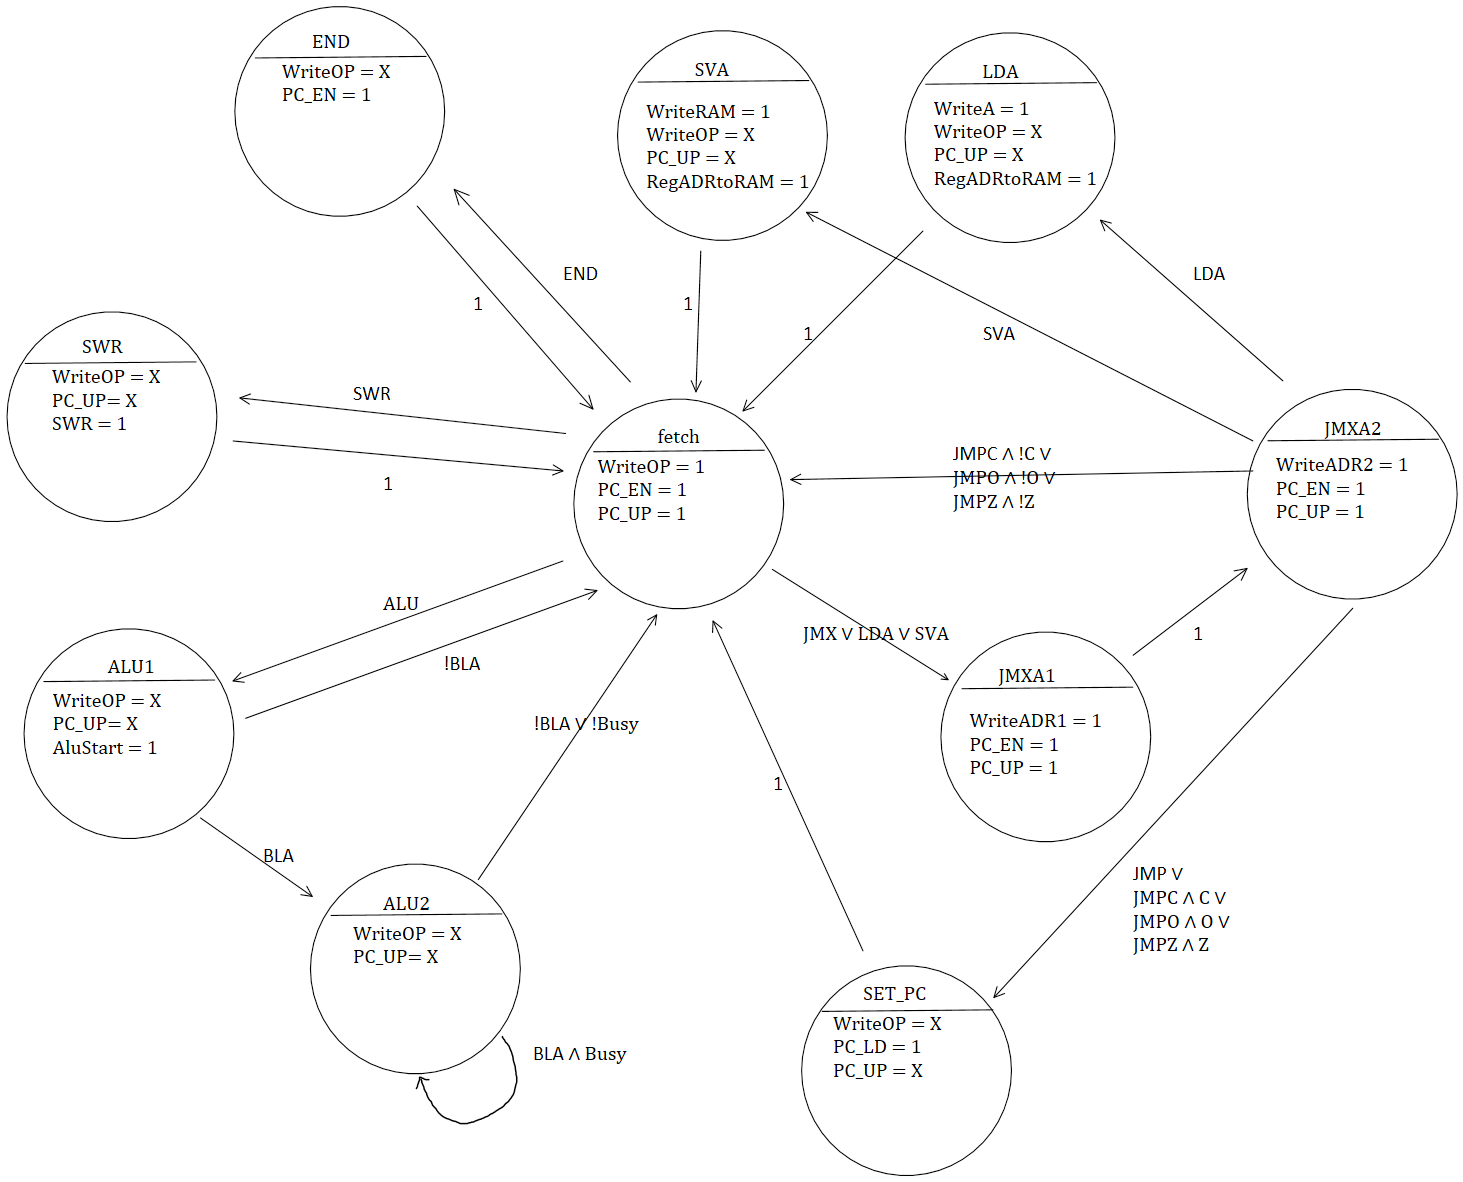
\includegraphics[scale=0.279]
    {content/figures/SW_Zustaende}
    \caption{Zustandsautomat Steuerwerk}
    \label{fig:SW_Zustaende}
\end{figure}


\section{Zustandscodierung}
\label{sec:Zustandscodierung}

\begin{table} [H]
    \centering
    \begin{tabular}{|l|c|c|c|c|}
        \hline
        \multirow{2}{*}{\textbf{Zustand}} & \multicolumn{4}{c}{\textbf{Codierung}}                \\

                                          & Q3                                     & Q2 & Q1 & Q0 \\
        \hline
        \textbf{Fetch}                    & 0                                      & 0  & 0  & 0  \\
        \hline
        \textbf{SET\_PC}                  & 0                                      & 0  & 1  & 0  \\
        \hline
        \textbf{ALU1}                     & 0                                      & 1  & 0  & 0  \\
        \hline
        \textbf{ALU2}                     & 0                                      & 1  & 0  & 1  \\
        \hline
        \textbf{JMXA1}                    & 1                                      & 0  & 0  & 0  \\
        \hline
        \textbf{JMXA2}                    & 1                                      & 0  & 0  & 1  \\
        \hline
        \textbf{LDA}                      & 1                                      & 1  & 0  & 0  \\
        \hline
        \textbf{SVA}                      & 1                                      & 1  & 0  & 1  \\
        \hline
        \textbf{SWR}                      & 1                                      & 1  & 1  & 0  \\
        \hline
        \textbf{END}                      & 1                                      & 1  & 1  & 1  \\
        \hline
        \textbf{Don´t Care}               & -                                      & -  & -  & -  \\
        \hline
    \end{tabular}
    \caption{Zustandscodierung des Steuerwerks}
    \label{tab:Zustandscodierung}
\end{table}

\noindent \textbf{Wichtig} Alle nicht definierten Zustände sind "Don´t Care"


\section{Operationen und Anweisungen}
Das Steuerwerk kann Mithilfe der ALU folgende Funktionen ausführen:
\begin{itemize}
    \item \textbf{Logisch} AND, OR, NOT
    \item \textbf{Arithmetisch} Addition (ADD), Subtraktion (SUB), Multiplikation (MUL).
    \item \textbf{Sprung} JMP, JMPC (für Carry), JMPO (für Overflow), JMPZ (für Zero).
    \item \textbf{Speicher} LDA (Load Register A), SVA (Save Register A).
    \item \textbf{Spezial} SWR (Switch Registers), END.
\end{itemize}

\noindent Dabei wird jede Operation durch eine Kombination der Steuerbits \texttt{C3..0} definiert.

\begin{table}[H]
    \centering
    \begin{tabular}{|p{0.5cm}|p{0.5cm}|p{0.5cm}|p{0.5cm}|p{2.7cm}|p{6cm}|}
        \hline
        \multicolumn{4}{|c|}{\textbf{Codierung}} & \textbf{Operation} & \textbf{Beschreibung}                                                                                                                         \\

        C3                                       & C2                 & C1                    & C0 &          &                                                                                                       \\
        \hline
        0                                        & 0                  & 0                     & 0  & AND      & Bitweises UND (\boldmath{$A \land B$})                                                                \\
        \hline
        0                                        & 0                  & 0                     & 1  & OR       & Bitweises ODER (\boldmath{$A \lor B$})                                                                \\
        \hline
        0                                        & 0                  & 1                     & 0  & NOT      & Invertiert A (\boldmath{$\neg A$})                                                                    \\
        \hline
        0                                        & 0                  & 1                     & 1  & ADD      & Binäre Addition (\boldmath{$A + B$})                                                                  \\
        \hline

        \hline
        0                                        & 1                  & 0                     & 0  & SUB      & Binäre Subtraktion (\boldmath{$A - B$})                                                               \\
        \hline
        0                                        & 1                  & 0                     & 1  & MUL      & Binäre Multiplikation (\boldmath{$A \times B$})                                                       \\
        \hline
        0                                        & 1                  & 1                     & 0  & RESERVED & \textit{Frei im PROM der ALU programmierbar}                                                          \\
        \hline
        0                                        & 1                  & 1                     & 1  & RESERVED & \textit{Frei im PROM der ALU programmierbar}                                                          \\
        \hline
        \hline
        1                                        & 0                  & 0                     & 0  & JMP      & \textbf{TODO}                                                                                         \\
        \hline
        1                                        & 0                  & 0                     & 1  & JMPC     & \textbf{TODO}                                                                                         \\
        \hline
        1                                        & 0                  & 1                     & 0  & JMPO     & \textbf{TODO}                                                                                         \\
        \hline
        1                                        & 0                  & 1                     & 1  & JMPZ     & \textbf{TODO}                                                                                         \\
        \hline

        \hline
        1                                        & 1                  & 0                     & 0  & LDA      & Schreibt den 4-Bit Operanden vom RAM in Register A (\boldmath{$RAM3..0 \rightarrow A$})               \\
        \hline
        1                                        & 1                  & 0                     & 1  & SVA      & Schreibt das 4-Bit Ergebnis von Register A in den RAM (\boldmath{$A \rightarrow RAM3..0$})            \\
        \hline
        1                                        & 1                  & 1                     & 0  & SWR      & Tauscht den Inhalt von Register A und Register B (\boldmath{$A \rightarrow B \land B \rightarrow A$}) \\
        \hline
        1                                        & 1                  & 1                     & 1  & END      & \textbf{TODO}  Beenden der Rechnenoperation                                                           \\
        \hline
    \end{tabular}
    \caption{Unterstützte Operationen}
    \label{fig:Unterstützte Operationen}
\end{table}






\input{content/Architektur-Übersicht.tex}

\chapter{Ablauf}

\chapter{Teststrategie für das Steuerwerk und die ALU}
\label{chap:Testen}


\section{Vorgehen zum Testen}

\begin{figure}[H]
    \centering
    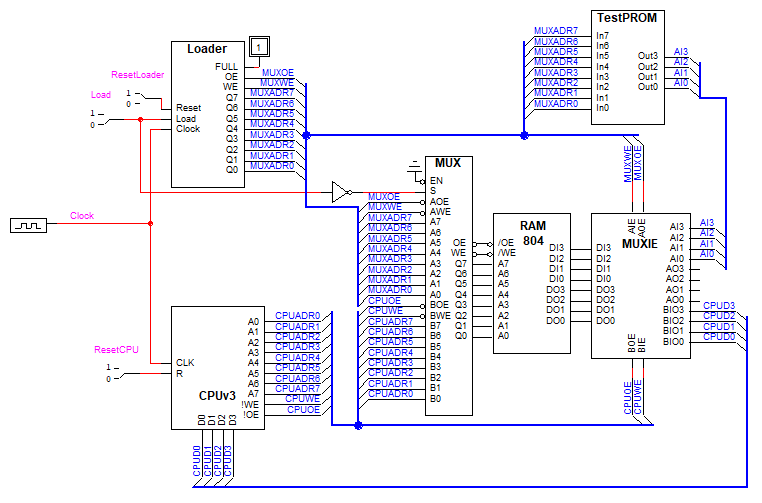
\includegraphics[width=0.9\textwidth]{content/figures/Testautomat.png}
    \caption{Testautomat zur Verifikation von Steuerwerk und RAM}
    \label{fig:Testautomat}
\end{figure}

Die folgende Schaltung wurde entwickelt, um das Steuerwerk und den RAM innerhalb der CPU zu validieren. Die Hauptkomponenten und ihr Zusammenspiel zur Testdurchführung können wie folgt beschrieben werden:

\begin{enumerate}
    \item \textbf{Loader:} Der Loader lädt Daten oder Programme in den Speicher (RAM). Über die Signale \texttt{Load} und \texttt{Clock} wird der Ladevorgang gesteuert. Der Reset-Eingang (\texttt{ResetLoader}) ermöglicht das Zurücksetzen des Loaders.
    \item \textbf{TestPROM:} Das Test-ROM speichert vordefinierte Testdaten oder Programme, die für die Verifizierung des Systems verwendet werden. Die Daten werden über Multiplexer an die restlichen Komponenten weitergeleitet.
    \item \textbf{Multiplexer (MUX und MUXIE):}
          \begin{itemize}
              \item Der \textbf{MUX} entscheidet, ob Adress- und Datensignale vom Loader oder der CPU stammen.
              \item Der \textbf{MUXIE} leitet Daten korrekt zwischen CPU, RAM und anderen Komponenten weiter.
          \end{itemize}
    \item \textbf{RAM:} Der Speicher (RAM 804) dient als Hauptspeicher für die Datenverarbeitung und speichert sowohl Programm- als auch Datensignale.
    \item \textbf{CPU:} Die CPU führt die Testprogramme aus und greift auf den Speicher zu. Über den Reset-Eingang (\texttt{ResetCPU}) kann die CPU zurückgesetzt werden.
\end{enumerate}

\section{Ziel der Tests}
Die Teststrategie zielt darauf ab, die korrekte Funktionalität des Steuerwerks und der ALU zu validieren. Folgende Bereiche stehen im Fokus:
\begin{itemize}
    \item Funktionalität des RAMs
    \item Ausführung von Steuerwerk-Befehlen
    \item Korrektheit logischer und arithmetischer ALU-Operationen
    \item Verarbeitung von mehrstufigen und iterativen Berechnungen
\end{itemize}

\section{Testkategorien und Testfälle}

\subsection{1. Variablen-Tests}
\noindent\textbf{Ziel:} Überprüfung der Funktionalität des RAMs durch Lesen und Schreiben von Werten. \\
\textbf{Programmzeilen:}
\begin{verbatim}
00 END
\end{verbatim}
\textbf{Erwartetes Ergebnis:} Adressen: 1--31; Werte: 0xF (für alle Adressen).

\begin{table}[H]
    \centering
    \rotatebox{90}{
        \begin{tabular}{|p{3cm}|p{6cm}|p{3cm}|p{3cm}|}
            \hline
            \textbf{Ziel}                                                                & \textbf{Eingaben und Programm}               & \textbf{Erwartetes Ergebnis} & \textbf{Status} \\ \hline
            Überprüfung der Funktionalität des RAMs durch Lesen und Schreiben von Werten & Adressen: 1--31; Werte: 0xF; \texttt{00 END} & Adressen: 1--31; Werte: 0xF  & succeeded       \\ \hline
        \end{tabular}
    }
    \caption{Testfall für Variablen-Tests}
\end{table}

\clearpage
\subsection{2. Steuerwerk-Befehle}
\noindent\textbf{Ziel:} Validierung von Steuerwerk-Befehlen wie Laden, Speichern und Springen. \\

\begin{table}[H]
    \centering
    \rotatebox{90}{
        \begin{tabular}{|p{2.5cm}|p{6.5cm}|p{3cm}|p{3cm}|}
            \hline
            \textbf{Befehl} & \textbf{Eingaben und Programm}                                                                                                                                 & \textbf{Erwartetes Ergebnis}                & \textbf{Status} \\ \hline
            LDA und SVA     & Adressen: 20--22; Werte: 0xA, 0xB, 0xC; \texttt{00 LDA 20, 03 SVA 23, 06 LDA 21, 09 SVA 24, 0B LDA 22, 0F SVA 25, 12 END}                                      & Adressen: 23--25; Werte: 0xA, 0xB, 0xC      & succeeded       \\ \hline
            SWR             & Adressen: 20--23; Werte: 0xA, 0xB, 0xC, 0xD; \texttt{00 LDA 20, 03 SWR, 04 LDA 21, 07 SWR, 08 SVA 24, 0B LDA 22, 0E SWR, 12 LDA 23, 15 SWR, 16 SVA 26, 25 END} & Adressen: 24--27; Werte: 0xA, 0xB, 0xC, 0xD & succeeded       \\ \hline
            JMP             & Adressen: 20--21; Werte: 0xA, 0xB; \texttt{00 LDA 20, 03 SVA 22, 06 SVA 23, 09 SVA 24, 12 JMP 27, 15 LDA 21, 18 SVA 22, 21 SVA 23, 24 SVA 24, 27 END}          & Adressen: 22--24; Werte: 0xA, 0xA, 0xA      & succeeded       \\ \hline
        \end{tabular}
    }
    \caption{Testfälle für Steuerwerk-Befehle}
\end{table}

\subsection{3. ALU-Befehle}
\noindent\textbf{Ziel:} Validierung der ALU-Operationen wie Addition, Subtraktion, AND, OR. \\

\begin{table}[H]
    \centering
    \rotatebox{90}{
        \begin{tabular}{|p{2.5cm}|p{6.5cm}|p{3cm}|p{3cm}|}
            \hline
            \textbf{Befehl} & \textbf{Eingaben und Programm}                                                                                         & \textbf{Erwartetes Ergebnis}      & \textbf{Status} \\ \hline
            AND             & Adressen: 20--21; Werte: 0xA, 0xF; \texttt{00 LDA 20, 03 SWR, 04 LDA 21, 07 AND, 08 SVA 22, 11 END}                    & Adresse 22: 0xA                   & succeeded       \\ \hline
            OR              & Adressen: 20--21; Werte: 0xA, 0x5; \texttt{00 LDA 20, 03 SWR, 04 LDA 21, 07 OR, 08 SVA 22, 11 END}                     & Adresse 22: 0xF                   & succeeded       \\ \hline
            ADD             & Adressen: 20--21; Werte: 0x2, 0x3; \texttt{00 LDA 20, 03 SWR, 04 LDA 21, 07 ADD, 08 SVA 22, 11 END}                    & Adresse 22: 0x5                   & succeeded       \\ \hline
            MUL             & Adressen: 20--21; Werte: 0x5, 0x5; \texttt{00 LDA 20, 03 SWR, 04 LDA 21, 07 MUL, 08 SVA 22, 11 SWR, 12 SVA 23, 15 END} & Adressen: 22--23; Werte: 0x1, 0x9 & succeeded       \\ \hline
        \end{tabular}
    }
    \caption{Testfälle für ALU-Befehle}
\end{table}

\subsection{4. Konditionelle Sprungbefehle}
\noindent\textbf{Ziel:} Validierung der konditionellen Sprungbefehle wie Jump-Zero, Jump-Overflow und Jump-Carry. \\

\begin{table}[H]
    \centering
    \rotatebox{90}{
        \begin{tabular}{|p{2.5cm}|p{6.5cm}|p{3cm}|p{3cm}|}
            \hline
            \textbf{Befehl} & \textbf{Eingaben und Programm}                                                                                                       & \textbf{Erwartetes Ergebnis} & \textbf{Status}                         \\ \hline
            Jump-Zero       & Adressen: 20--21; Werte: 0x5, 0x5; \texttt{00 LDA 20, 03 SWR, 04 LDA 21, 07 SUB, 08 SVA 22, 0B JMZ 14, 0E LDA 20, 11 SVA 22, 14 END} & Adresse 22: 0x5              & succeeded                               \\ \hline
            Jump-Overflow   & Adressen: 20--21; Werte: 0xF, 0xD; \texttt{00 LDA 20, 03 SWR, 04 LDA 21, 07 ADD, 08 SVA 22, 0B JMO 14, 0E LDA 21, 11 SVA 22, 14 END} & Adresse 22: 0x4              & failed : test-case might include errors \\ \hline
            Jump-Carry      & Adressen: 20--21; Werte: 0xF, 0x1; \texttt{00 LDA 20, 03 SWR, 04 LDA 21, 07 ADD, 08 SVA 22, 0B JMC 14, 0E LDA 21, 11 SVA 22, 14 END} & Adresse 22: 0x0              & succeeded                               \\ \hline
        \end{tabular}
    }
    \caption{Testfälle für konditionelle Sprungbefehle}
\end{table}

\subsection{5. Kombinatorische Tests}
\noindent\textbf{Ziel:} Sicherstellung der korrekten Verarbeitung komplexer Operationen. \\

\begin{table}[H]
    \centering
    \rotatebox{90}{
        \begin{tabular}{|p{2.5cm}|p{6.5cm}|p{3cm}|p{3cm}|}
            \hline
            \textbf{Testfall}    & \textbf{Eingaben und Programm}                                                                                                                                                             & \textbf{Erwartetes Ergebnis}      & \textbf{Status} \\ \hline
            Mehrstufige Addition & Adressen: 20--23; Werte: 0x1, 0x2, 0x3, 0x4; \texttt{00 LDA 20, 03 SWR, 04 LDA 21, 07 ADD, 08 SVA 24, 11 SWR, 12 LDA 22, 15 ADD, 16 SVA 25, 19 SWR, 20 LDA 23, 23 ADD, 24 SVA 26, 27 END}  & Adressen: 24--26; Werte: 3, 6, 10 & succeeded       \\ \hline
            Iterative Berechnung & Adressen: 20--22; Werte: 0x2, 0x5, 0x1; \texttt{00 LDA 20, 03 SVA 23, 06 LDA 22, 09 SWR, 0A LDA 21, 0D SUB, 0E SVA 21, 11 JMZ 1E, 14 LDA 20, 17 SWR, 18 LDA 23, 1B ADD, 1C JMP 06, 1F END} & Adresse 23: 0xA                   & succeeded       \\ \hline
        \end{tabular}
    }
    \caption{Testfälle für kombinatorische Tests}
\end{table}

\chapter{Changelog}
\label{chap:Changelog}



\appendix

\end{document}
